% ======== Plantilla para elaboracion de informes ========
% version: 3.0  - Julio/2015 
% autores:
%   Jorge Pérez Zerpa - Pedro Curto - Mihdí Caballero
% Comentarios y sugerencias en el foro del taller:
%   https://eva.fing.edu.uy/course/view.php?id=307
% ========================================================
%
% ----- INSTRUCCIONES -----
% Abrir archivos README.txt incluido en *.zip
% -------------------------
%
% ----- LICENCIA -----
% Este trabajo es distribuido bajo la licencia LaTeX Project Public License
% Puede y DEBE ser usado, modificado y distribuido gratuitamente.
% ---------------------
%
% ========================================================

% --- Comentarios ---
% Durante todo el archivo se ven comentarios escritos con porcentaje al inicio
% dado que LaTeX es un lenguaje de programacion compilado, los comentarios
% no tienen valor ninguno para el compilador pero si para el programador (humano). Esto puede ser útil para agregar descripciones para el usuario mientras elabora un documento o si es realizado entre varias personas.
% --------------------

% --- Clase de archivo ---
% Con este comando se define que tipo de documento vamos a hacer
% en este caso un articulo, en una hoja a4 y con tamanio de fuente 11pt.
\documentclass[a4paper,11pt]{article}
% los tamanios mas utilizados son 10,11 y 12 pt y representan un tamanio de referencia, o sea que al cambiar a 12 pt todos los textos van a aumentar proporcionalmente, al estilo homotecia.


% A partir de aqui se definiran ciertos paquetes o funciones a ser utilizadas
% dentro del documento.


% --- codificacion de archivo ---
% El paquete inputenc sirve para que el compilador pueda interpretar los acentos en espaniol de forma estandar, dependiendo del sistema operativo hay que darle una configuracion diferente:
%
%para windows se escribe:
%\usepackage[ansinew]{inputenc}
%-
%para linux se escribe:
%\usepackage[latin1]{inputenc}
% o
\usepackage[utf8]{inputenc}
%-
%para mac se escribe:
%\usepackage[applemac]{inputenc}

%
% ----------------------------------


% --- idioma ---
% El paquete babel sirve para separar correctamente las palabras en muchos idiomas, aquií­ esta configurado con espaniol (spanish). Tambien sirve para que el Ií­ndic etenga tií­tulo "Indice" en lugar de "Contents".
\usepackage[spanish]{babel} 
% --------------


% --- Fuentes ---
% El paquete fontenc sirve para controlar las fuentes que utiliza el documento
\usepackage[T1]{fontenc}
% Si dejamos comentado el paquete de abajo utilizaremos la fuente por defecto
% si se quita el comentario se usa sans. Se puede usar times, y otras opciones que se dejan comentadas. 
%\usepackage{sans}
%\usepackage{fbb}
%\usepackage{bera}
%\usepackage{sans}
%\usepackage{times}
%\usepackage{libertine} 


\usepackage{dirtytalk} % Paquete para facilitar la notación de citas con el comando \say{}



% --- Gráficos ---
% El paquete graphicx sirve para controlar figuras con \includegraphics.
\usepackage{graphicx}
% Esta linea indica el lugar (path) en el cual se encuentra la carpeta donde colocamos imágenes, para ahorrar colocarlo en cada
% llamado de una imagen en el documento.
\graphicspath{{./figuras/}}
% Estos paquetes permiten colocar varias figuras en el entorno "figure" como subfiguras (cualquiera de los dos).
\usepackage{float}
\usepackage{subfig} 


% --- Lenguaje matemático ---
% fuentes para escribir sí­mbolos
\usepackage{amsfonts,amssymb,amsthm,amsmath}


% --- Tablas ---
% Paquetes para el manejo de tablas, creación de filas y columnas unidas.
\usepackage{multirow} 
\usepackage{multicol} 
% Control de color en tablas muy versátil.
\usepackage[table]{xcolor}


% --- Hipervínculos ---
% paquete para marcar los hiperví­nculos en i­ndice y referencias
\usepackage{hyperref}
% Para citar referencias  
\usepackage{cite} 
\hypersetup{colorlinks, urlcolor=cyan, citecolor=green, linkcolor=blue} % Pinta con color las referencias
\usepackage[hypcap]{caption} % Las imágenes tienen hiperreferencia y se ven completas y no solo la leyenda. 
% Para hacer hiperreferencias a páginas web
\usepackage{url} 


\usepackage{booktabs} 

% --- Numeración ---
% Paquete que cambia como se representa la numeración de las imágenes, ecuaciones y tablas
\usepackage{chngcntr}
% Ahora se nombran por sección reiniciando el conteo en cada sección
\counterwithin{figure}{section}
\counterwithin{equation}{section}
\counterwithin{table}{section}


% Para agregar al índice las refencias
\usepackage[nottoc,notlot,notlof]{tocbibind} 



% Aqui comienzan los datos del trabajo. El comando \date{\today} asigna la fecha en que se compila como la fecha del trabajo, tambien se puede escibe directamente, ej. \date{5 de setiembre de 2012}.

\title{Template introductorio a \LaTeX ~en formato informe} % El simbolo "~" genera un espacio entre \LaTeX y el texto que sigue
\author{%
  Nombres de autores\\ %
  Grupo de estudiantes, Facultad y/o Universidad a la que pertenece el autor.}
\date{\today}
% ------------------------

%\pagestyle{empty}
% ====================================


%El paquete colortbl sirve para darle color a las tablas
\usepackage{colortbl}

% Este paquete se utiliza para generar texto de relleno.
\usepackage{blindtext}

% este paquete determina que el texto tenga como fuente normal: times, consultar el eva de latex para mas opciones.
%\usepackage{times}


% ===== Encabezado =====
% esta es una posible configuración para el encabezado. 
%Si se comentan estas dos lineas no habrá encabezado y la numeración de página aparecerá abajo de cada hoja. En la página donde se llame a \maketitle no se coloca encabezado.
\pagestyle{myheadings}
\markright{Universidad de la República \hfill Introducción a \LaTeX \hfill}
% ======================


%% ===== Ajuste layout pagina =====
% define el ancho del texto en la hoja
\setlength{\textwidth}{155mm}
% define el alto del texto en la hoja
\setlength{\textheight}{210mm}
% los márgenes pueden ser editador con
\oddsidemargin=-.25cm
%% ================================

% --- commandos definidos a gusto del usuario ---
\newcommand{\ds}{\displaystyle}
\def\x{{\bf x}}

\newcommand{\subfigureautorefname}{\figureautorefname}

% -----------------

% =====================================================
% =====================================================




% =====================================================
% ========  Aca comienza el cuerpo del texto ==========
%
\begin{document}
	
% Se renuevan comandos ya existentes de LaTeX como se desee, en este caso del nombre de tablas y figuras.	
\renewcommand{\tablename}{\bfseries Tabla} % Cambia nombre de tablas
\renewcommand{\figurename}{\bfseries Figura} % Cambia nombre de figuras 
%\newcommand{\subfigureautorefname}{\figureautorefname} % Para que al referenciar una subfigura aparezca "Figura"	
% Se refiere a las tablas y figuras con el comando \autoref{label} para que aparezca referenciado automáticamente el nombre de lo referenciado (Tabla o Figura) continuado por el número de la misma.	
%
% El comando \verb+maketitle+ sirve para escribir la cabecera con los datos del trabajo (título, autor y fecha).
\maketitle


% resumen
\begin{abstract}
En este párrafo se presenta un breve resumen del documento, es opcional y es particularmente usado en publicaciones en revistas. Para no colocarlo basta con comentar el párrafo. %
Generalmente se utilizan unas pocas líneas para describir el trabajo. %
En este documento presentaremos ejemplos de uso de \LaTeX~para escribir un documento y le daremos un formato tipo informe.
\end{abstract}

% índice
\tableofcontents

% para separar la carátula del texto introducimos un salto de pagina
\newpage

% definimos una sección con el comando section

\section{Introducción}
%
Las secciones son numeradas usando un formato por defecto aunque también puede ser configurable a gusto del usuario.

Para rellenar un poco de texto vamos a escribir cosas sin sentido: cosas sin sentido, cosas sin sentido. Incluso usando el paquete \verb+blindtext+ podemos generar texto automático como el siguiente párrafo.

\blindtext

\section{Marco Teórico}
%
En esta sección presentaríamos un marco teórico del contenido del trabajo, generalmente debe ser lo mínimo indispensable para obtener los resultados y concluir.

En nuestro caso serán secciones sobre mas temas de \LaTeX.

\subsection{Fuentes}

En \LaTeX se puede escribir con diferentes fuentes, sin embargo hay que saber controlarlas. En esta sección se muestran algunos ejemplos\footnote{En esta sección aprovechamos e introducimos el manejo de notas al pie.}.

%\times
Este es un ejemplo de otro tipo de fuente, en este caso caligráfica. Para poder escribir es necesario poner el paquete que controla las fuentes (fontenc) y el paquete de letra caligráfica (calligra).

Este es otro ejemplo de otro tipo de fuente, en este caso ``Carolingan Miniscules``. El paquete de letra es carolmin.

\normalfont
En la página ''http://www.tug.dk/FontCatalogue/alphfonts.html`` hay un catálogo muy extenso de fuentes para usar en \LaTeX. 

Para insertar hipervínculos podemos usar dos comandos en particular: href para esconder la ruta del hipervínculo bajo un texto

\href{http://www.tug.dk/FontCatalogue/alphfonts.html}{texto del Link}

o el comando url para mostrar directamente la ruta
\url{http://www.tug.dk/FontCatalogue/alphfonts.html}

\subsection{Tablas}
Los tablas son comunes en los trabajos científicos, sirven para representar datos de forma compacta. Vamos a mostrar un ejemplo de un tabla.

\subsubsection{Ejemplos}
\label{ej_fonts}
En el \autoref{cuadro_1} se muestra un ejemplo tomado de una tesis que trata sobre motores de combustión interna, particularmente los que siguen el ciclo de Otto. Tambien, se muestra como ejemplo un detalle que algunas veces puede pasar desapercibido, ya que no se utiliza comúnmente. Desde mi punto de vista es uno de los pocos inconveniente que tiene LaTeX que todavía no está solucionado. Me refiero a la nota al pie dentro de las tablas, que muchas veces son necesarias. Pero lamentablemente al día de hoy hay que ponerlas manualmente, en esta tabla se presenta un ejemplo de cómo se hace.

\begin{table}[!ht]
\centering
\caption[Aquí se escribe el comentario que se pone en el índice]{Este es el comentario de la tabla, donde se da una explicación detallada sobre el contenido del mismo.}
\label{cuadro_1}
\medskip 
\begin{tabular}{lc}
\hline \hline
 $r$, relación de compresión & $10$ \\
 $B$, diámetro interior del cilindro &  $79.5 \times 10^{-3}$ m\\
 $V_0$, volumen muerto de la cámara & $49.639 \times 10^{-6}$ m$^3$\\
 $T_w$, temperatura de la pared del cilindro & $600$ K\\
$T_1$, temperatura de entrada$^{\dag}$ & $333$ K\\
 $h$, coeficiente de transferencia de calor$^{\dag}$ & $1305$ W/m$^2$K\\
 $m$, masa de la mezcla de gases dentro del cilindro$^{\ddag}$ & $4.176\times 10^{-4}$ kg \\
\hline \hline
\end{tabular}
\flushleft
\footnotesize
$^{\dag}$ Sólo para TTF.
\\
$^{\ddag}$ Como condición inicial para la simulación numérica y fija para TTF.
\end{table}

Otro ejemplo de tabla en donde se pintan de un color diferente algunas columnas y se muestra cómo hacer columnas múltiples. El color en las tablas no se ve bien, pero si se compila en pdf se ve mejor.
\begin{table}[!ht]
\centering
\caption{Ejemplo de una tabla que muestra columnas múltiples y colores diferentes.}
\label{tab:cuadro_2}
\begin{tabular}{|c|cccc|}
\hline
 X/Y &  \multicolumn{4}{>{\columncolor[rgb]{0.8, 0.8, 0.8}}c|}{Población } \\ 
 Edad &  Montevideo &  Colonia & Salto & Rocha \\ 
\hline 
 20 &  23 &  34 &  56 & 87 \\ 
 25 &  22 &  56 &  76 & 23 \\ 
\hline 
\end{tabular}
\end{table}

Otro ejemplo de tabla es la \autoref{tab:presillas1}, en donde utilizamos el paquete \texttt{xcolor} para pintar intercaladamente las filas de la tabla.

\begin{table}[h]
	\centering
	\caption{Cantidad de presillas por barra.} \rowcolors{2}{}{gray!15} 
	\begin{tabular}{ccccccc}
		\textbf{Barra} & \textbf{L (m)} & \boldmath$\lambda_{max}$ & \boldmath$r_i$ \textbf{(cm)} & \boldmath$a_{max}$ \textbf{(cm)} & \textbf{nº presillas} & \boldmath$a_{final}$ \textbf{(cm)} \\
		\hline
		\hline
		\textbf{1} & 3.30  & 136   & 2.43  & 247.50 & 2     & 110.00 \\    \hline
		\textbf{2} & 3.30  & 136   & 2.43  & 247.50 & 2     & 110.00 \\    \hline
		\textbf{3} & 3.30  & 136   & 2.43  & 247.50 & 2     & 110.00 \\    \hline
		\textbf{4} & 3.30  & 136   & 2.43  & 247.50 & 2     & 110.00 \\    \hline
	\end{tabular}%
	\label{tab:presillas1}%
\end{table}%

En la \autoref{tab:conectividad} se presenta otro estilo de tablas, en donde se utilizan distintos espesores de línea además de columnas múltiples. Notar que al hacer columnas múltiples se especifica en la celda creada si se quiere tener lineas verticales a los lados.

\begin{table}[h]
	\centering
	\caption{Conectividad de elementos.} 
	\begin{tabular}{|c|c|c|}
		\toprule[0.8mm]                                                                 
		\multicolumn{3}{|c|}{Element's conectivity    }  \\  
		\midrule[0.5mm]                                  
		Element & Start & End \\ \midrule[0.5mm]                                                                                                                                                     
		1 &    1 &    2 \\
		2 &    2 &    3 \\
		3 &    3 &    4 \\
		4 &    4 &    5 \\
		\bottomrule[0.8mm]                                        
	\end{tabular}%
	\label{tab:conectividad}%
\end{table}%                                



\section{Desarrollo}
%
El desarrollo sería una de las partes centrales de un informe o artículo... en este caso presentaremos ejemplos de creación de fórmulas matemáticas con \LaTeX.

\subsection{Fórmulas matemáticas}
Hay varias maneras de insertar una fórmula matemática en un trabajo. Primero y más fácil es en la misma línea, como por ejemplo: $E=mc^{2}$. También se puede hacer en una línea aparte, sin numerar de esta forma $$E=mc^{2}$$ después se pueden poner en una línea aparte y numerarlas, de esta forma: 
\begin{equation}\label{ec:Ein}
  E=mc^{2}
\end{equation} %
%
cuando se escribe en el entorno \say{equation} es conveniente no dejar un renglón en blanco entre el texto y el entorno, así LaTeX dejará el espacio adecuado a cada fórmula. Nótese que se utiliza aquí el paquete \texttt{dirtytalk}, en donde \say{se pueden colocar citas \say{dentro de} otras citas}. Se pueden hacer referencias a todas las etiquetas creadas, por ejemplo a la ecuación~\eqref{ec:Ein} o al \autoref{tab:cuadro_2}, incluso a la sección~\ref{ej_fonts}.


\subsection{Imágenes}
%
La \autoref{fig:optimo} es una figura de ejemplo, para un formato de la figura jpg, es necesario compilar el documento con el compilador PDFLaTeX, para formatos de figura eps, se puede compilar en Latex.
\begin{figure}[h!]
\centering
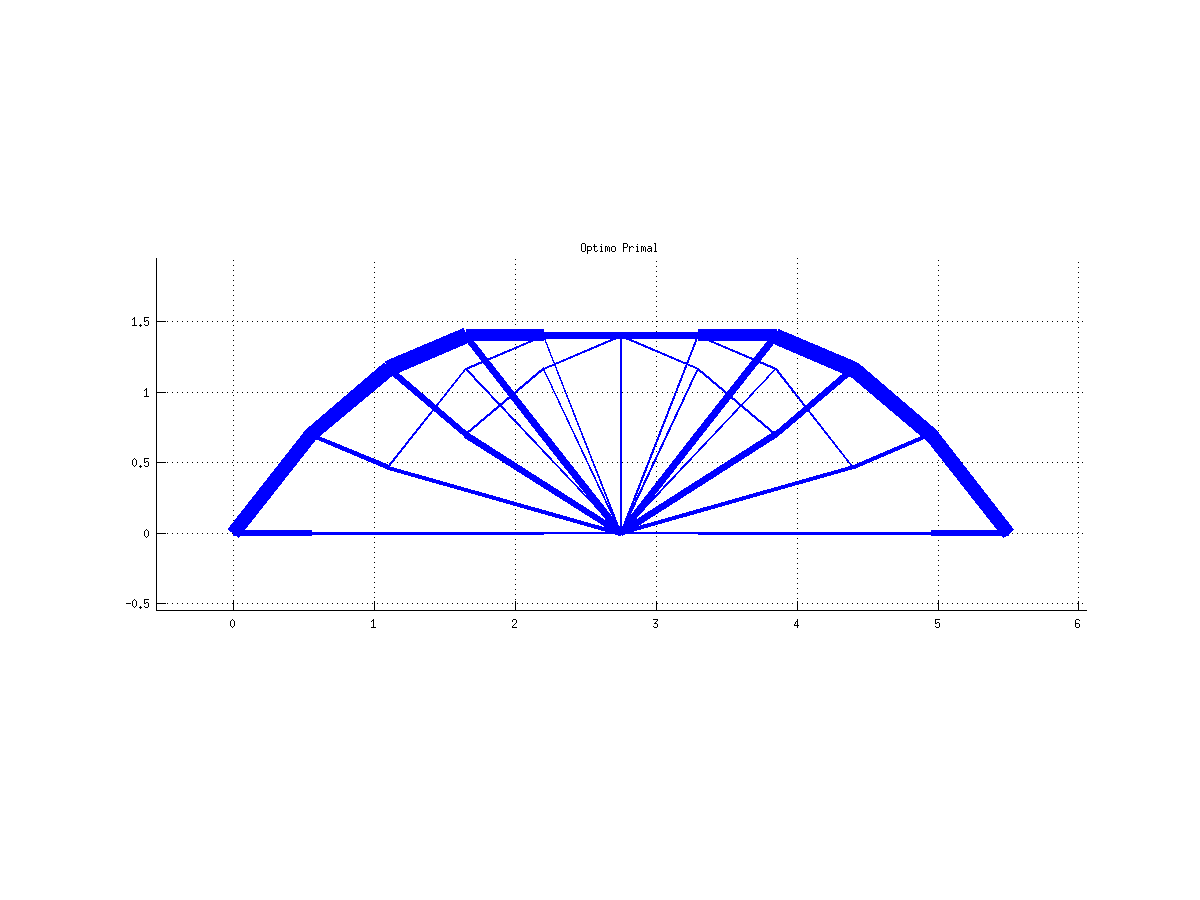
\includegraphics[width=1\textwidth]{figuras/optimo_primal}
\label{fig:optimo}
\caption{}
\end{figure}


Se puede referenciar a cada figura del subfigure por ejemplo \autoref{fig:matesub}.\\

\begin{figure}[htb]
    \centering
    \subfloat[surf]
    {
        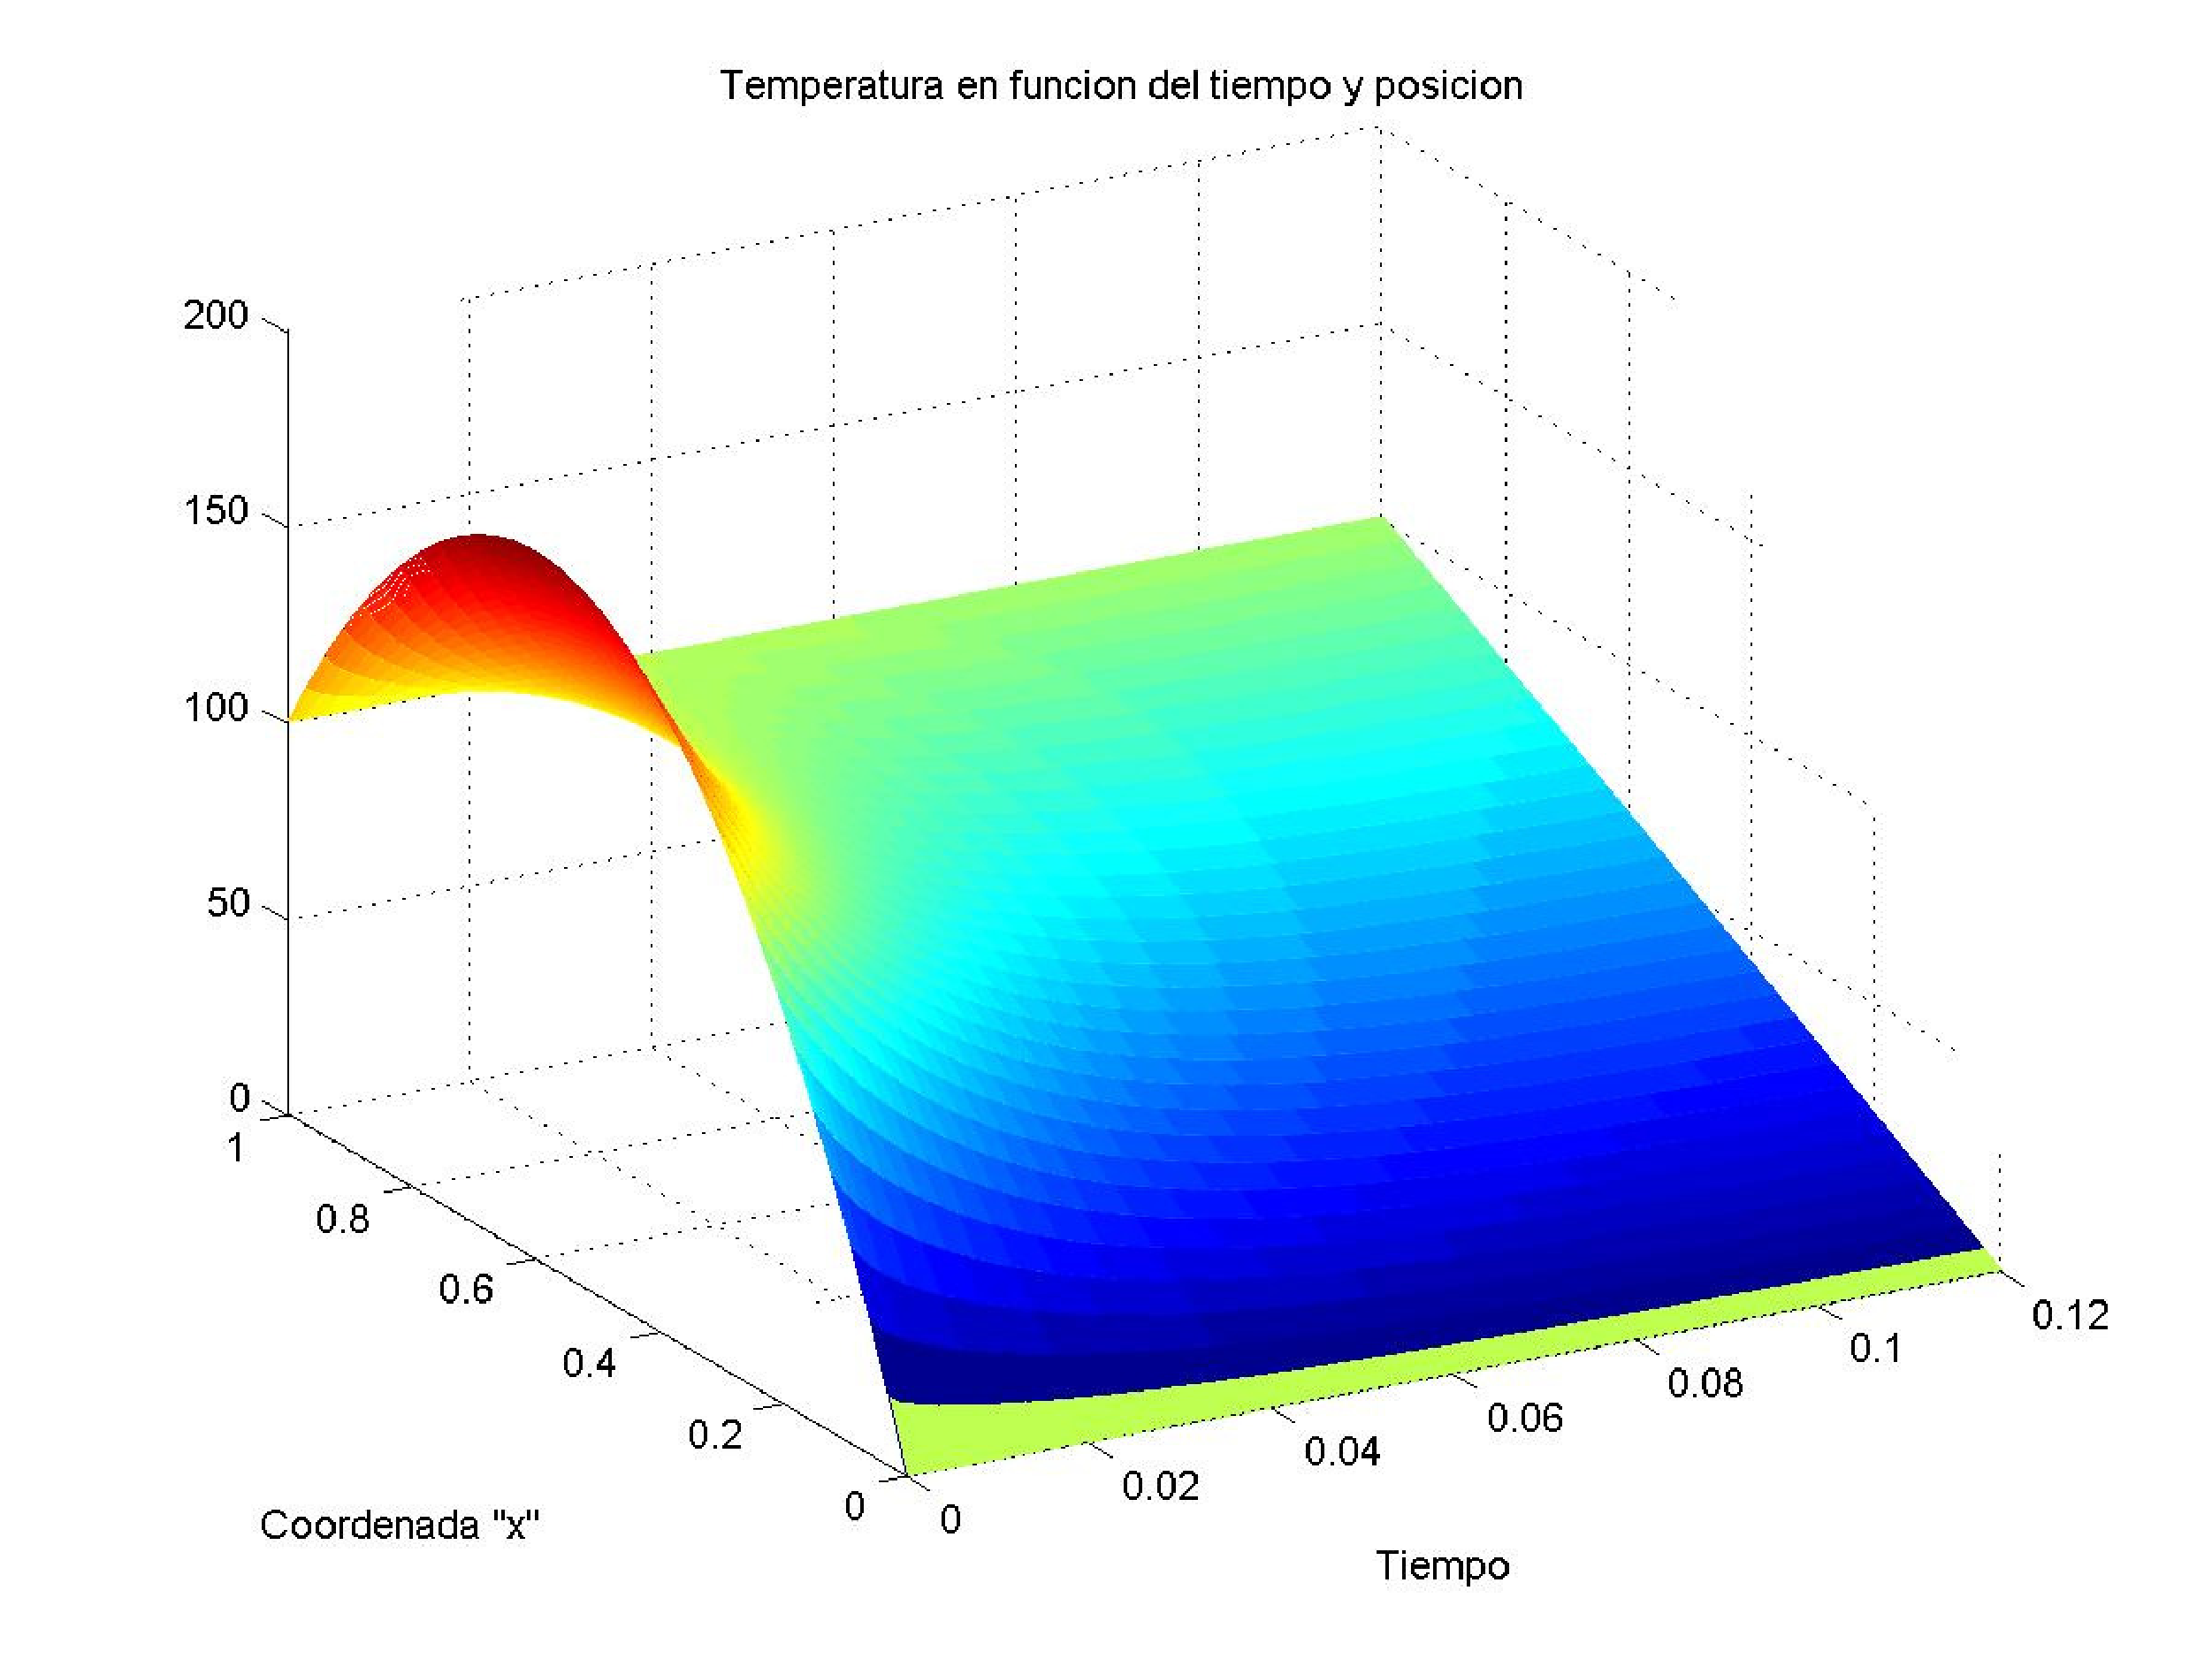
\includegraphics[width=0.4\textwidth]{surf}
        \label{fig:surfsub}
    }
    \hfil
    \subfloat[Esta es la imagen infrarroja de un mate junto a un termo donde se puede ver el reflejo de la radiación.]
    {
        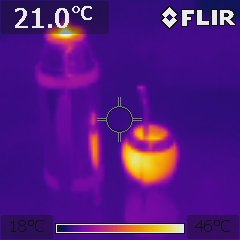
\includegraphics[width=0.3\textwidth]{mate}
        \label{fig:matesub}
    }
    \caption{Ejemplo de dos figuras usando subfigure.}
%    \label{fig:mapasej1_CECENR}
\end{figure}




\begin{minipage}[b]{0.45\textwidth}
También pueden ser incluidas figuras en formato pdf como por ejemplo en la Figura~\ref{fig:matesub} y \autoref{fig:surfsub}, que si vemos en el directorio figuras confirmamos que es un archivo pdf. El entorno minipage es útil para colocar figuras o texto en columnas, como se ve en este caso.  
    \end{minipage}
    %
    \hfil
    %    \pause
    %
    \begin{minipage}{0.45\textwidth}
        \begin{center}
            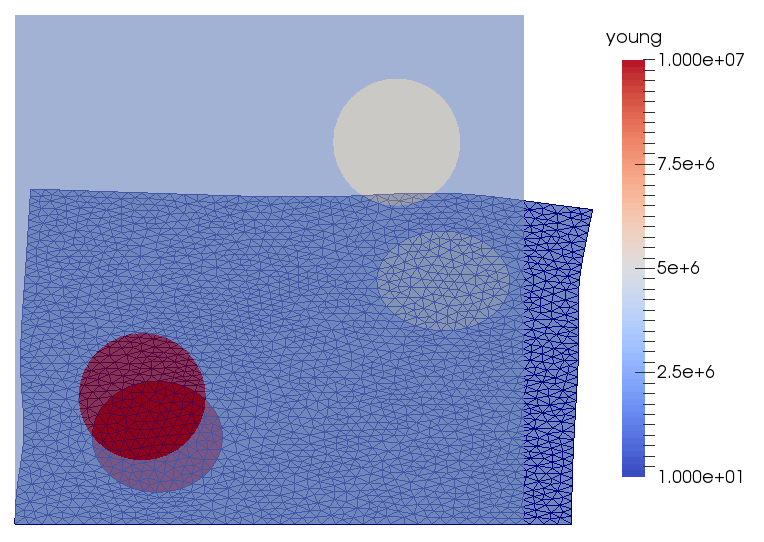
\includegraphics[width=1\textwidth]{chapa10}
        \end{center}
    \end{minipage}





\newpage

% ========================
\section{Conclusiones}
%
Aquí irían las conclusiones del artículo.  Tal vez se quieran mostrar conclusiones de forma esquemática como items... comoesto
%
\begin{itemize}
  \item Conclusión numero 1... 
  \item otra conclusión.
\end{itemize}

o también enumerándolas

\begin{enumerate}
  \item item primero...
  \item item segundo...
\end{enumerate}


\subsection{Citación de bibliografía}
%
Es posible citar artículos utilizados como referencia utilizando la función ``cite''. Por ejemplo citamos el libro \cite{lamport94} utilizando la etiqueta lamport94 que fue definida previamente al final del archivo latex como se puede ver en el código de este ejemplo. %
%
Se pueden citar tantos artículos como se quiera siempre que estén incluidos en el archivo \cite{otraetiqueta}. Existen otras formas mas complejas de citar en trabajos grandes como tesis o libros, utilizando archivos .bib . % ver http://en.wikibooks.org/wiki/LaTeX/Bibliography_Management
%


% =====================
\begin{thebibliography}{15}

\bibitem{lamport94}
  Leslie Lamport,
  \emph{\LaTeX: A Document Preparation System}.
  Addison Wesley, Massachusetts,
  2nd Edition,
  1994.

\bibitem{otraetiqueta}
  Otro autor,
  \emph{Título de artículo o libro}.
  Editorial o Journal,
  Edición o número de revista,
  Año.

\end{thebibliography}

% =====================

\end{document}
